\section{Results}

\subsection{Experimental setup}

% likzet: good
\paragraph{Datasets}
We conduct experiments across multiple datasets: 

\begin{itemize}
    \item Multiple choice question answering dataset MMLU-Pro~\cite{wang2024mmluprorobustchallengingmultitask},  widely adopted by the community as one of the main performance benchmarks. 
    It spans 14 domains, offering a broad selection of questions of varying complexities. 
    Each question has approximately ten options, with a single correct one, which eliminates ambiguity in evaluation.
    \item GSM8K (Grade School Math 8K)~\cite{cobbe2021gsm8k} - dataset of 8.5K high quality linguistically diverse grade school math word problems.
    \item MedMCQA~\cite{pmlr-v174-pal22a} - large-scale, Multiple-Choice Question Answering (MCQA) dataset designed to address real-world medical entrance exam questions. It has more than 194k high-quality AIIMS and NEET PG entrance exam MCQs covering 2.4k healthcare topics and 21 medical subjects are collected with an average token length of 12.77 and high topical diversity
\end{itemize}


\paragraph{LLMs}
Regarding the models \footnote{All models and datasets are published under permissive licenses that allow them to be used for research purposes}, we utilize a variety of open models to analyze how the trend changes with model size. 
At the same time, our focus is on smaller models for fine-tuning to make our results reproducible and more relevant to the distillation scenario.

We apply our pipeline to three models: 
Qwen2.5-3B, Phi-4-Mini, LLama 3.2 3B.
For them, we measure single token and chain-of-thought entropy, collect other response metadata, fine-tune the models, and evaluate the overall pipeline.

Bigger models are used to further extend the entropy aggregate and MASJ analysis: Mistral 24B, Phi-4, Mistral 123B \cite{mistral123b}.
For the chain-of-thought distillation we utilize an ensemble of models: DeepSeek-V3-0324 \cite{deepseekai2024deepseekv3technicalreport}, Qwen 3 235B, Llama 4 Maverick \cite{llama4}.

\subsubsection{Our method and baselines}

In experiments, we performed training for 10 or 20 epochs; see more information below.
In the case of the reasoning used during training, we split the training into two equal halves for the first and the second round of fine-tuning.

\paragraph{Pipeline (ours)} For easy and medium groups, we perform SFT for five epochs. For the hard group, we apply learning from a distilled chain-of-thought of a larger model for another five epochs.

\paragraph{Alternative} As the alternative approach, we perform SFT for five epochs for the hard group. Next, for easy and medium groups, we apply learning from a distilled chain-of-thought of a larger model for another five epochs.

\paragraph{SFT} As our first baseline, we train the model via SFT without the data split for 10 epochs. 

\paragraph{Curriculum} For the second baseline, we train the model via curriculum-based SFT: 3 epochs on easy data, 3 epochs on medium data, and 4 epochs on hard data. 

\paragraph{Distillation} As an idealistic target, we tuned the LLM via distillation without the data split for 10 epochs.

\subsubsection{Technical details}

Based on ROC AUC results and SFT's positive performance on medium and easy questions (see \ref{sec:sensitivity_study}), we use single-token entropy as our complexity metric for the pipeline described in Section~\ref{sec:pipeline}. 

We randomly split the data into train, validation, and test with a ratio of 70:10:20. Next, in each chunk, we balance the data so that the number of entries in each complexity group is equal. 
Since there are fewer hard questions, we filter out medium and easy ones to match the size of the hard group.


\subsection{Main results}
\label{sec:pipeline_results}

\begin{figure*}[ht]
    \centering
    \begin{subfigure}[b]{0.48\linewidth}
        \centering
        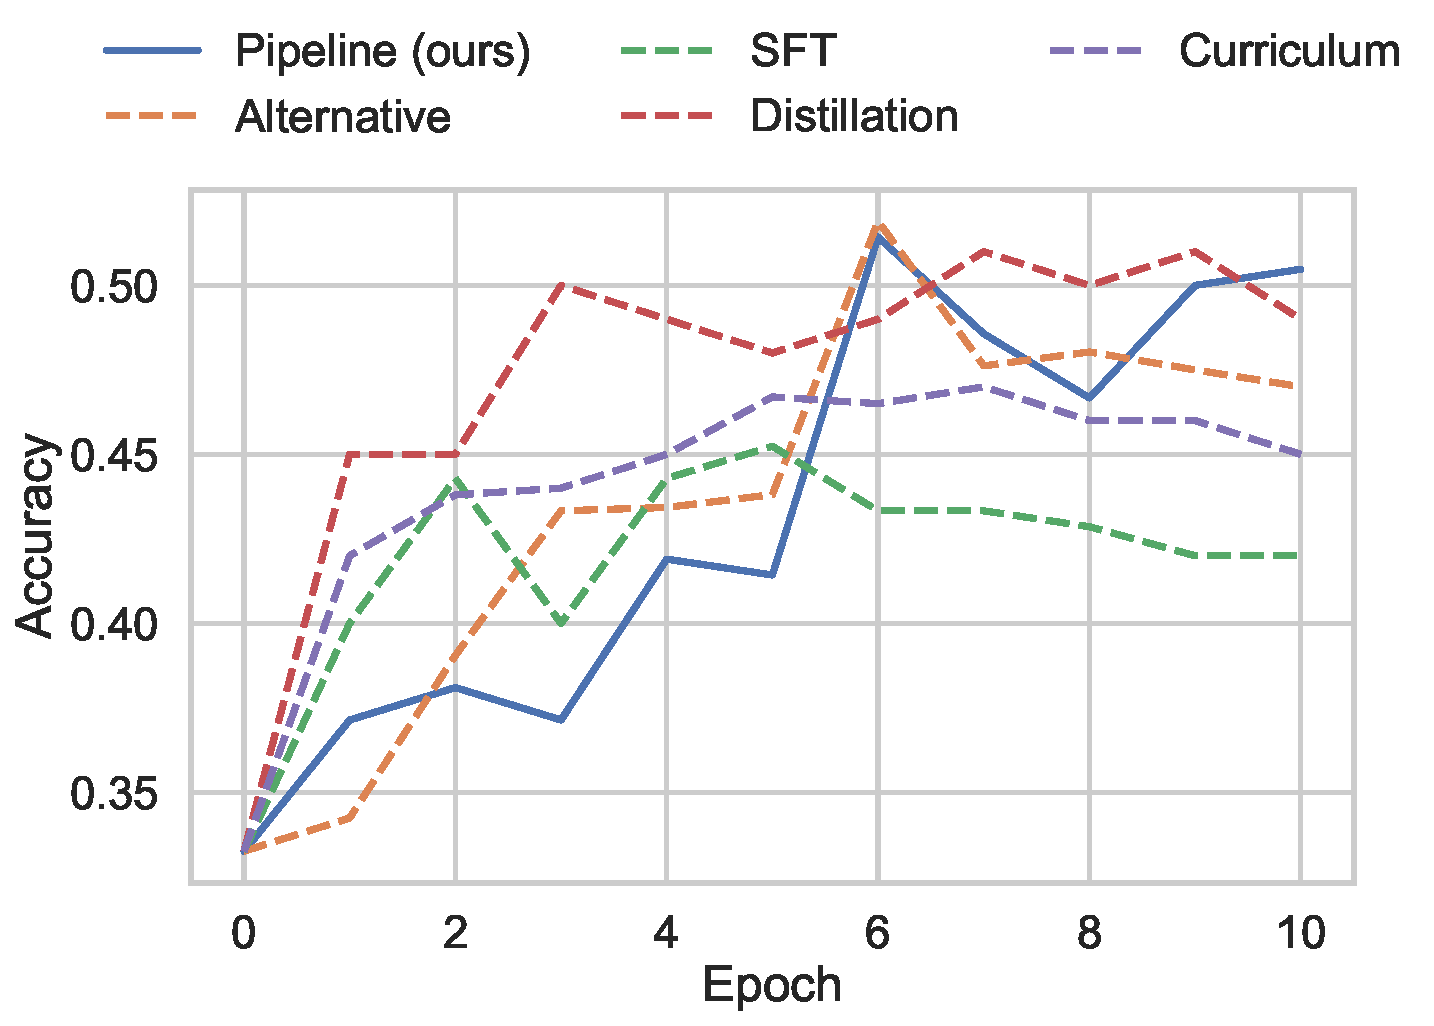
\includegraphics[width=1\linewidth]{images/qwen_pipeline.pdf}
        \caption{Accuracy for fine-tuning pipelines after 10 epochs for Qwen 3B (MMLU-Pro)}
        \label{fig:qwen_pipeline}
    \end{subfigure}
    \hfill
    \begin{subfigure}[b]{0.48\linewidth}
        \centering
        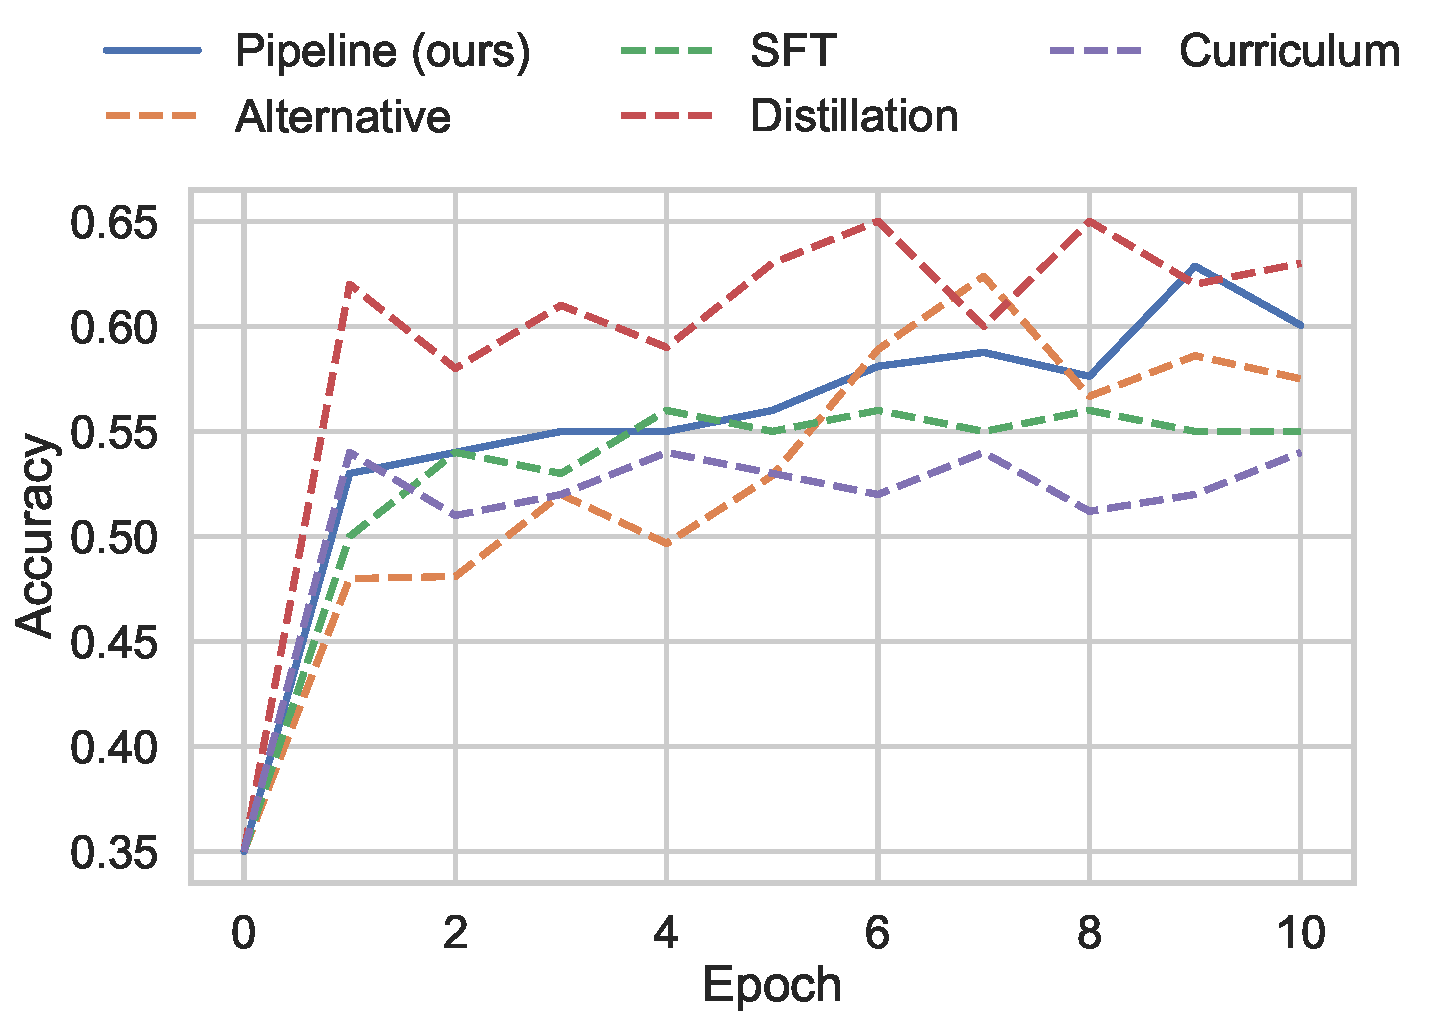
\includegraphics[width=1\linewidth]{images/phi_pipeline.pdf}
        \caption{Accuracy for fine-tuning pipelines after 10 epochs for Phi-4-mini (MMLU-Pro)}
        \label{fig:phi_pipeline}
    \end{subfigure}
\end{figure*}
\begin{figure*}[h]
    \centering
    \begin{subfigure}[b]{0.48\linewidth}
        \centering
        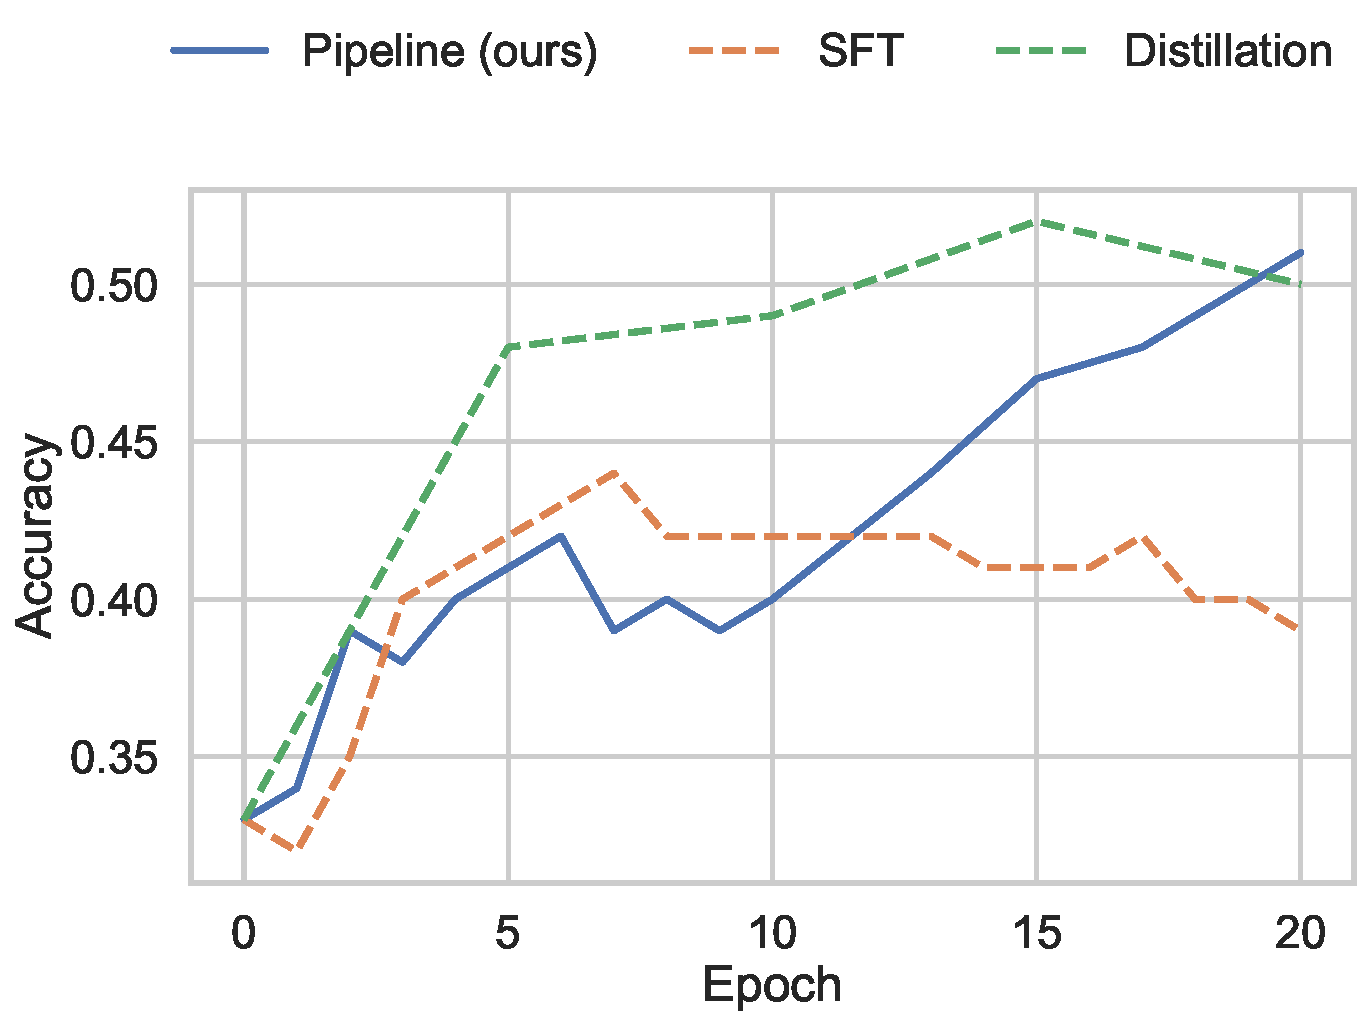
\includegraphics[width=1\linewidth]{images/qwen_pipeline_20epochs.pdf}
        \caption{Accuracy for fine-tuning pipelines after 20 epochs for Qwen 3B (MMLU-Pro)}
        \label{fig:qwen_pipeline_20epochs}
    \end{subfigure}
    \hfill
    \begin{subfigure}[b]{0.48\linewidth}
        \centering
        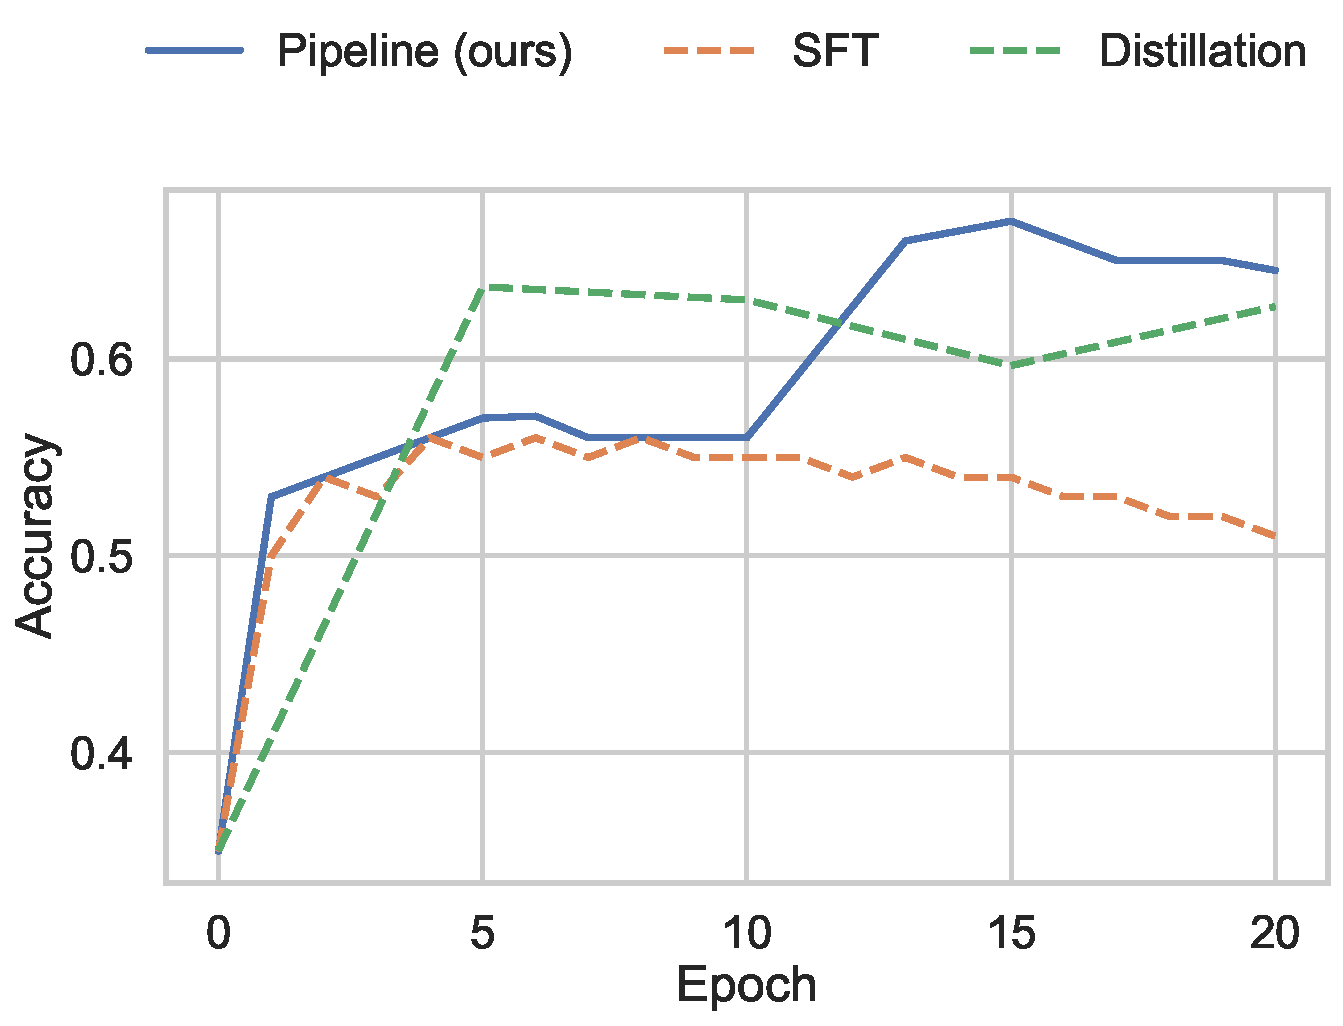
\includegraphics[width=1\linewidth]{images/phi_pipeline_20epochs.pdf}
        \caption{Accuracy for fine-tuning pipelines after 20 epochs for Phi-4-mini (MMLU-Pro)}
        \label{fig:phi_pipeline_20epochs}
    \end{subfigure}
\end{figure*}

Table ~\ref{tab:results_10epochs} and Figures ~\ref{fig:qwen_pipeline} ~\ref{fig:phi_pipeline} show the results for MMLU Pro. 
We see that the proposed training scheme results in a significant improvement over SFT, curriculum-based SFT, and an alternative training scheme that uses distillation for only easy and medium questions. 
Qwen 3B achieves an accuracy of 0.50 compared to 0.47 and 0.42 for alternative and baseline, respectively, while Phi-4-mini gets to 0.60 compared to 0.58 and 0.46.
At the same time, we see that the pipeline provides comparable performance to the distillation with significantly less data in the number of tokens processed. 
Qwen 3B achieves an accuracy of $0.50$ compared to $0.49$, saving $79\%$ tokens, while Phi-4-mini gets to $0.60$ compared to $0.63$, saving $82\%$ tokens. 
We can also detect an uptrend in the pipeline training, while the full distillation approach exhibits the signs of a plateau. 

To confirm the plateau trend, we ran an extended set of experiments over 20 epochs with the same training split. Table~\ref{tab:results_20epochs} and Figures ~\ref{fig:qwen_pipeline_20epochs} ~\ref{fig:phi_pipeline_20epochs} show the results. 
We find an even stronger confirmation of the previous findings with the proposed scheme outperforming all baselines. 
Qwen 3B achieves an accuracy of $0.52$ compared to $0.50$ and $0.39$ for distillation and baseline, respectively, while Phi-4-mini gets to $0.64$ compared to $0.63$ and $0.51$. 
The same data savings of $79\%$ and $82\%$ apply.

To confirm that the method generalizes to other datasets and models, we perform the same experiments for GSM8K and MedMCQA datasets across two models: LLama 3.2 3B and Phi-4 mini. Table~\ref{tab:results_20epochs} shows the results.
We see that across both models and datasets, our pipeline achieves accuracy either comparable to or surpassing the distillation baseline, with significant data savings.

Training hyperparameters are provided in the Appendix \ref{sec:hyperparameters}.

\begin{table}[ht]
\centering
\begin{tabular}{l l l}
\hline
Method & Qwen 3B & Phi4-mini \\
\hline
SFT & 0.42 / 29k & 0.55 / 27k \\
Curriculum & 0.45 / 29k & 0.54 / 27k \\
Distillation & \underline{0.49} / 1.97m & \textbf{0.63} / 1.51m \\
Alternative & 0.47 / 1.5m & 0.58 / 1.2m  \\
Pipeline (ours) & \textbf{0.50} / \textbf{399k} & \underline{0.60} / \textbf{268k}  \\
\hline
\end{tabular}
\caption{Accuracy / tokens processed for complexity-aware fine-tuning pipelines after 10 epochs (MMLU Pro)}
\label{tab:results_10epochs}
\end{table}

\begin{table*}[ht]
\centering
\begin{tabular}{l cc cc cc}
\toprule
& \multicolumn{2}{c}{MMLU Pro} & \multicolumn{2}{c}{GSM8K} & \multicolumn{2}{c}{MedMCQA} \\
\cmidrule(lr){2-3} \cmidrule(lr){4-5} \cmidrule(lr){6-7}
Method & Qwen 3B & Phi4-mini & LLama 3B & Phi4-mini & LLama 3B & Phi4-mini \\
\midrule
SFT & 0.39 & 0.51 & 0.13 & 0.19 & 0.51 & 0.51 \\
Distillation & \underline{0.50} & \underline{0.63} & \underline{0.79} & \underline{0.89} & \underline{0.56} & \underline{0.57} \\
Pipeline (ours) & \textbf{0.52} & \textbf{0.64} & \textbf{0.82} & \textbf{0.89} & \textbf{0.56} & \textbf{0.58} \\
\bottomrule
\end{tabular}
\caption{Accuracy for complexity-aware fine-tuning pipelines after 20 epochs.}
\label{tab:results_20epochs}
\end{table*}

\subsection{Sensitivity study}
\label{sec:sensitivity_study}

\subsubsection{Alternative complexity estimates}

To analyze the appropriate fine-tuning methods for each complexity band, we first perform the standard SFT for each group.

The same data-splitting procedure described in Section \ref{sec:pipeline_results} is applied to MASJ reasoning score and single-token entropy as complexity metrics.

\begin{figure}[h]
    \centering
    \begin{subfigure}[b]{0.48\linewidth}
        \centering
        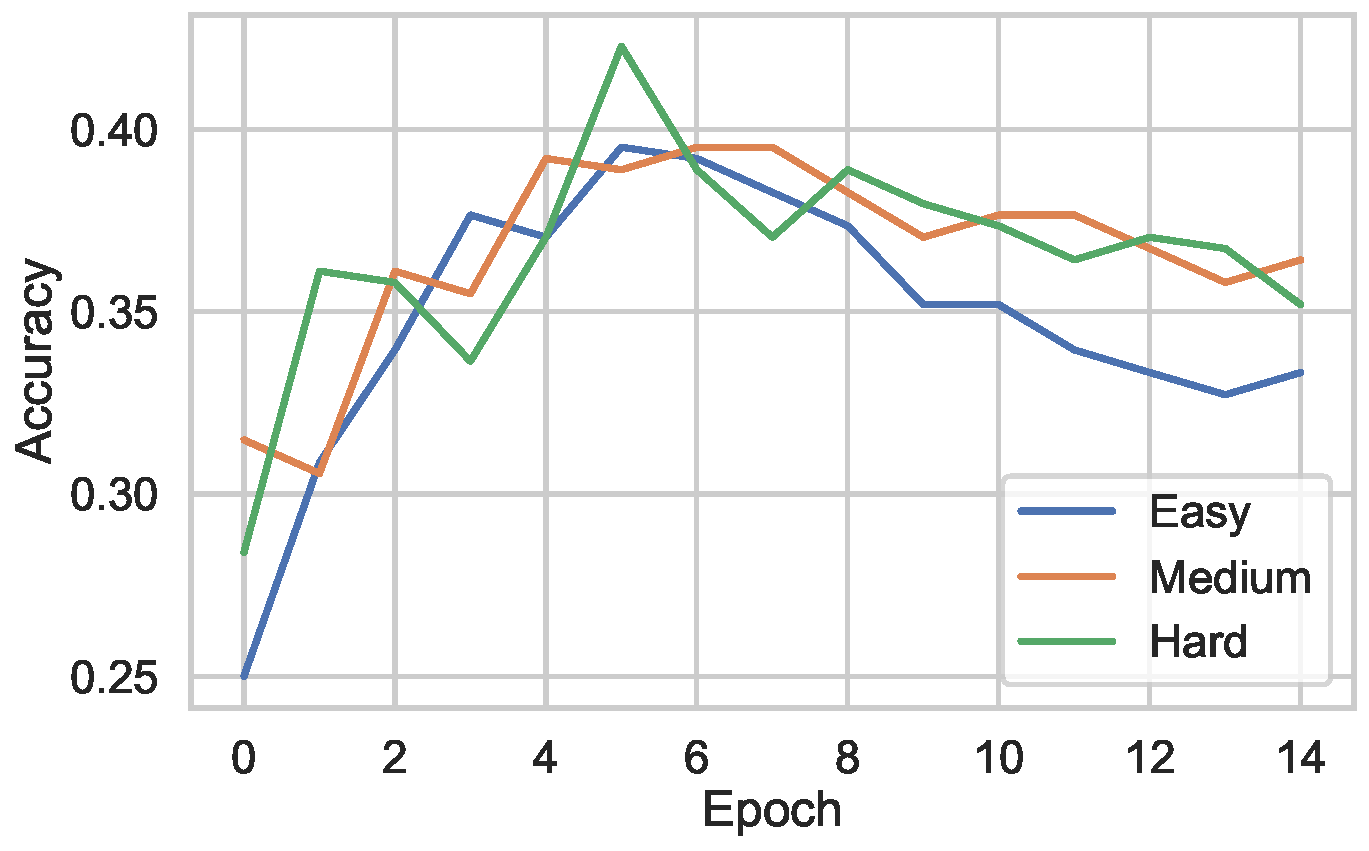
\includegraphics[width=\linewidth]{images/qwen3B_sft_masj_split.pdf}
        \caption{SFT by MASJ reasoning score (Qwen 3B)}
        \label{fig:sft_masj_reasoning_qwen3B}
    \end{subfigure}
    \hfill
    \begin{subfigure}[b]{0.48\linewidth}
        \centering
        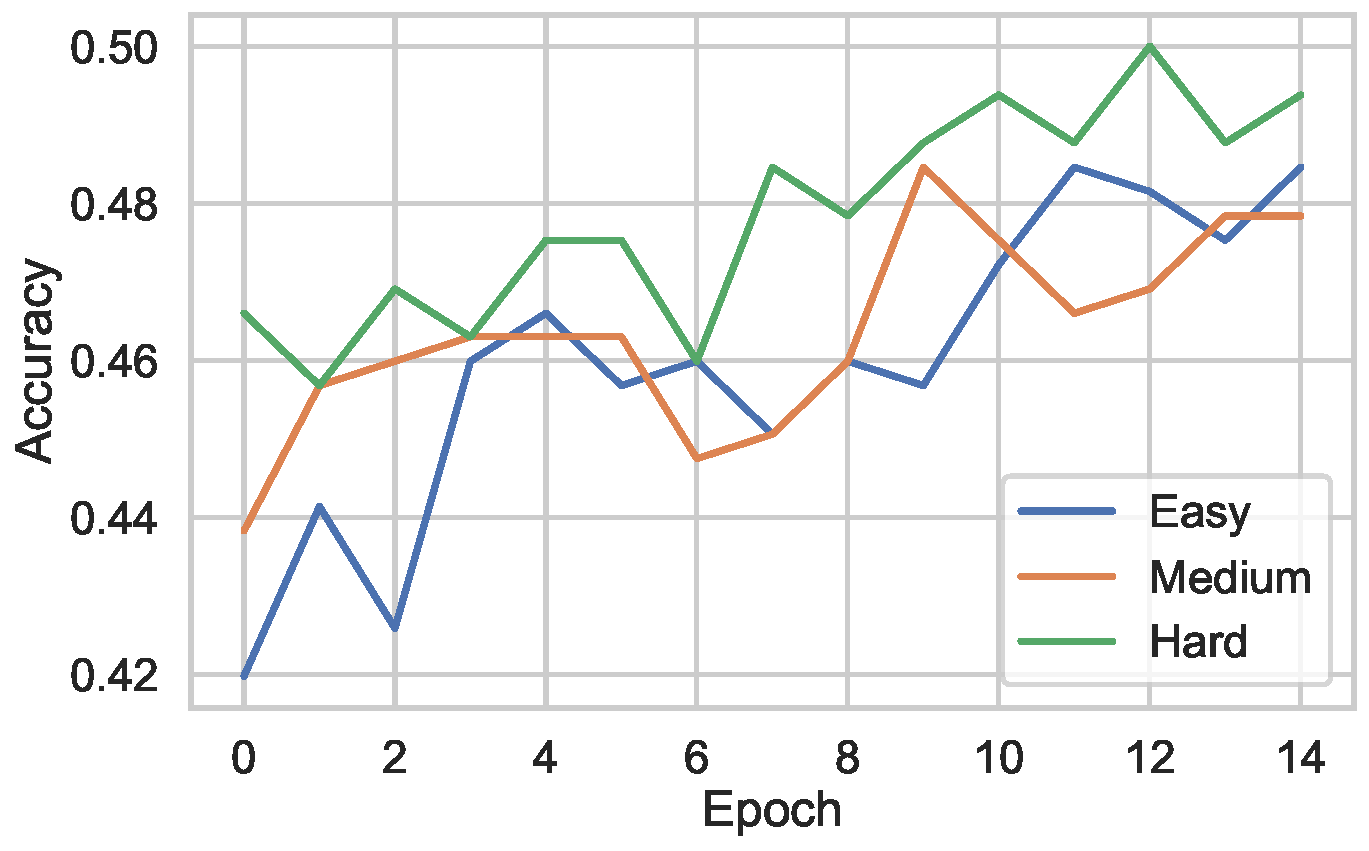
\includegraphics[width=\linewidth]{images/phi_sft_masj_split.pdf}
        \caption{SFT by MASJ reasoning score (Phi-4-mini)}
        \label{fig:sft_masj_reasoning_phi4mini}
    \end{subfigure}
    \hfill
    \begin{subfigure}[b]{0.48\linewidth}
        \centering
        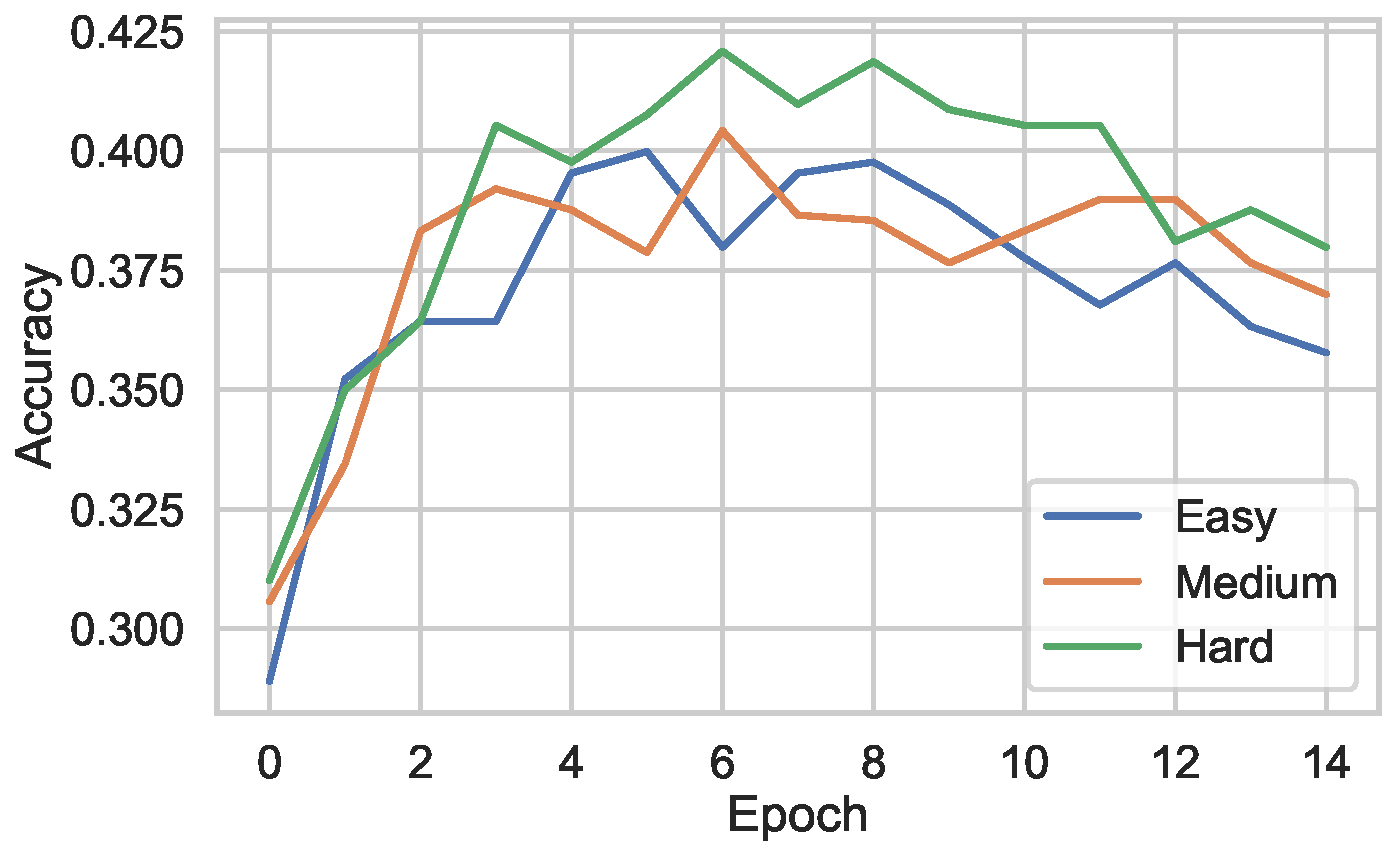
\includegraphics[width=\linewidth]{images/qwen3B_sft_entropy_split.pdf}
        \caption{SFT by single token entropy (Qwen 3B)}
        \label{fig:sft_entropy_qwen3B}
    \end{subfigure}
    \hfill
    \begin{subfigure}[b]{0.48\linewidth}
        \centering
        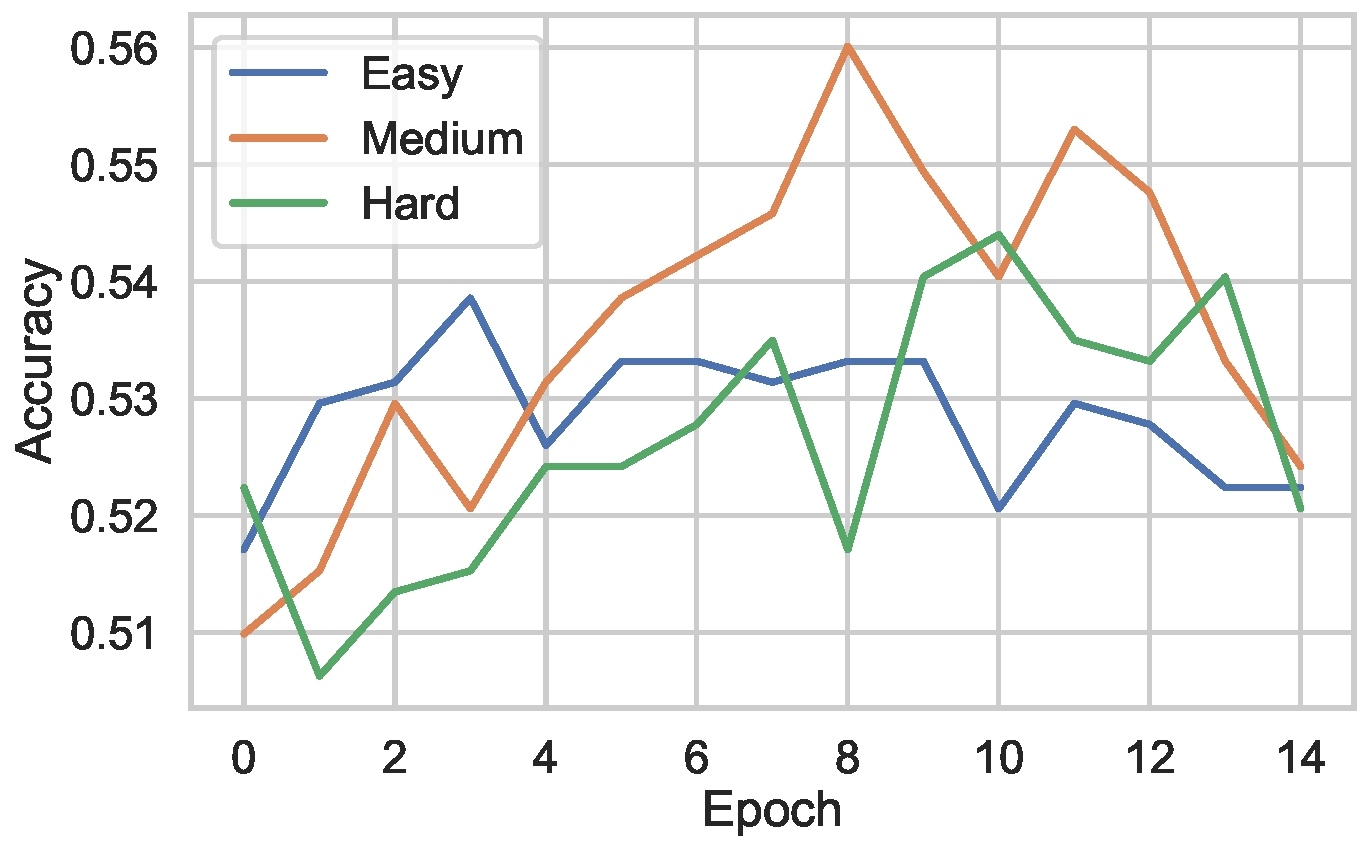
\includegraphics[width=\linewidth]{images/phi_sft_entropy_split.pdf}
        \caption{SFT by single token entropy (Phi-4-mini)}
        \label{fig:sft_entropy_phi4mini}
    \end{subfigure}
    \caption{SFT quality dynamics during training with split by complexity estimates provided  by the MASJ reasoning score and the single token entropy across Phi-4-mini and Qwen 3B models.}
    \label{fig:combined_sft_analysis}
\end{figure}

Figures \ref{fig:sft_entropy_phi4mini} \ref{fig:sft_entropy_qwen3B} show the results of SFT for each group split by the single-token entropy. For Phi-4-mini, we see that medium and easy questions outperform hard ones for the first 10 epochs. Shortly after, performance starts to decline for all groups.
For Qwen 3B, we do not see a significant difference between the groups. Moreover, the performance plateaus after five epochs.

Figures \ref{fig:sft_masj_reasoning_phi4mini} and \ref{fig:sft_masj_reasoning_qwen3B} show the results of SFT for each group split by the MASJ reasoning score. We do not see a strong difference in performance between the groups. In combination with questionable ROC AUC scores, provided in Table~\ref{tab:roc_auc_masj}, it makes MASJ reasoning score a less favorable metric for further experiments.

\begin{figure}[h]
    \centering
    \begin{subfigure}[b]{0.48\linewidth}
        \centering
        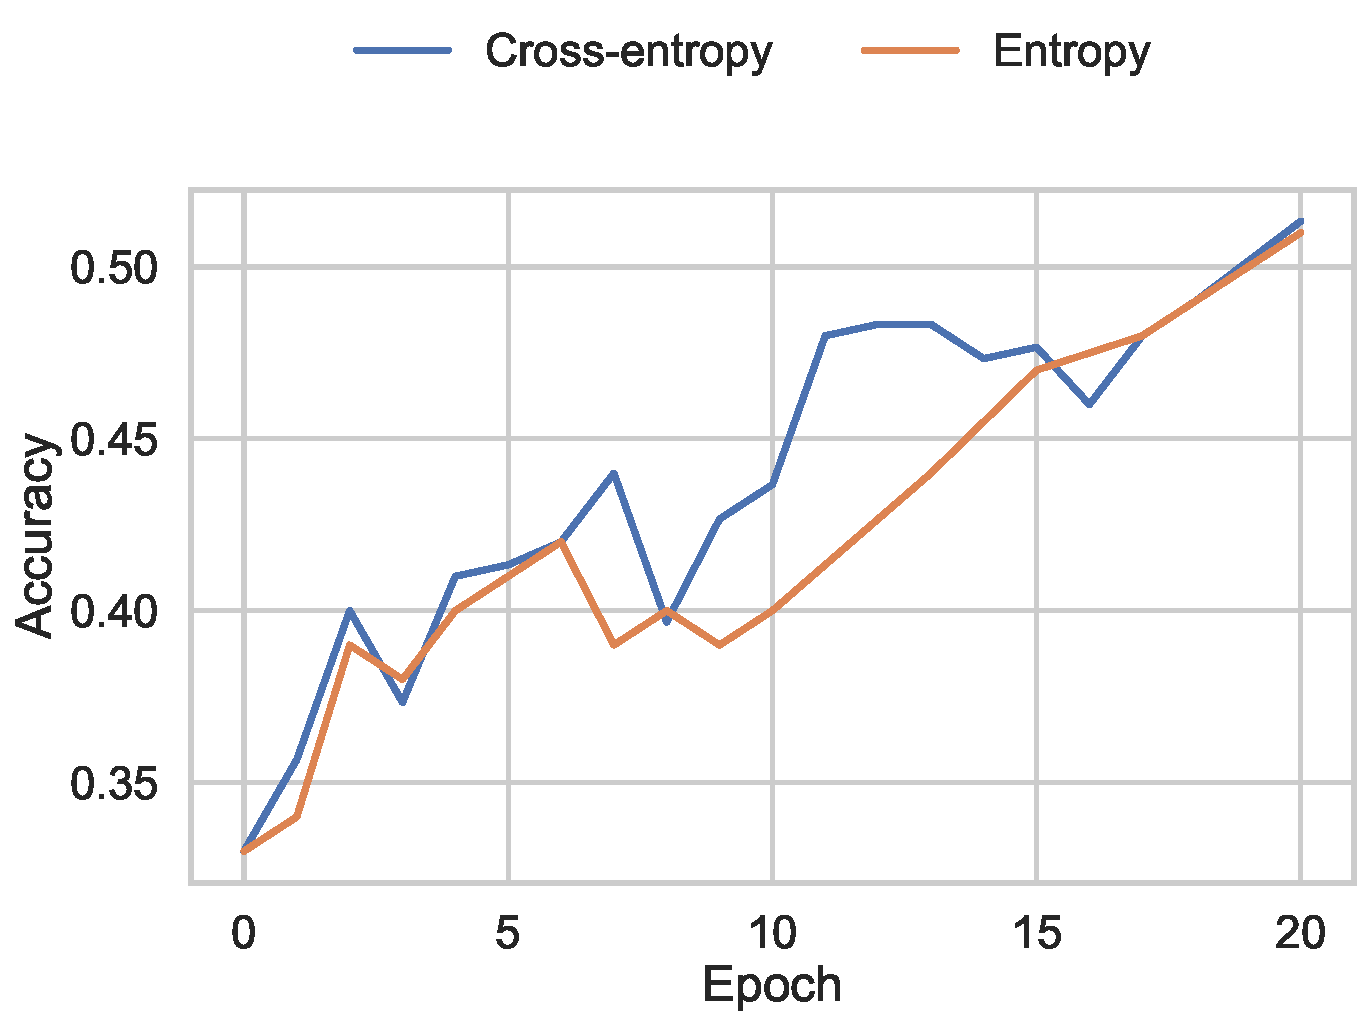
\includegraphics[width=\linewidth]{images/qwen_e_vs_ce.pdf}
        \caption{Pipeline performance with cross-entropy (Qwen 3B)}
        \label{fig:entropy_vs_crossentropy_qwen3B}
    \end{subfigure}
    \hfill
    \begin{subfigure}[b]{0.48\linewidth}
        \centering
        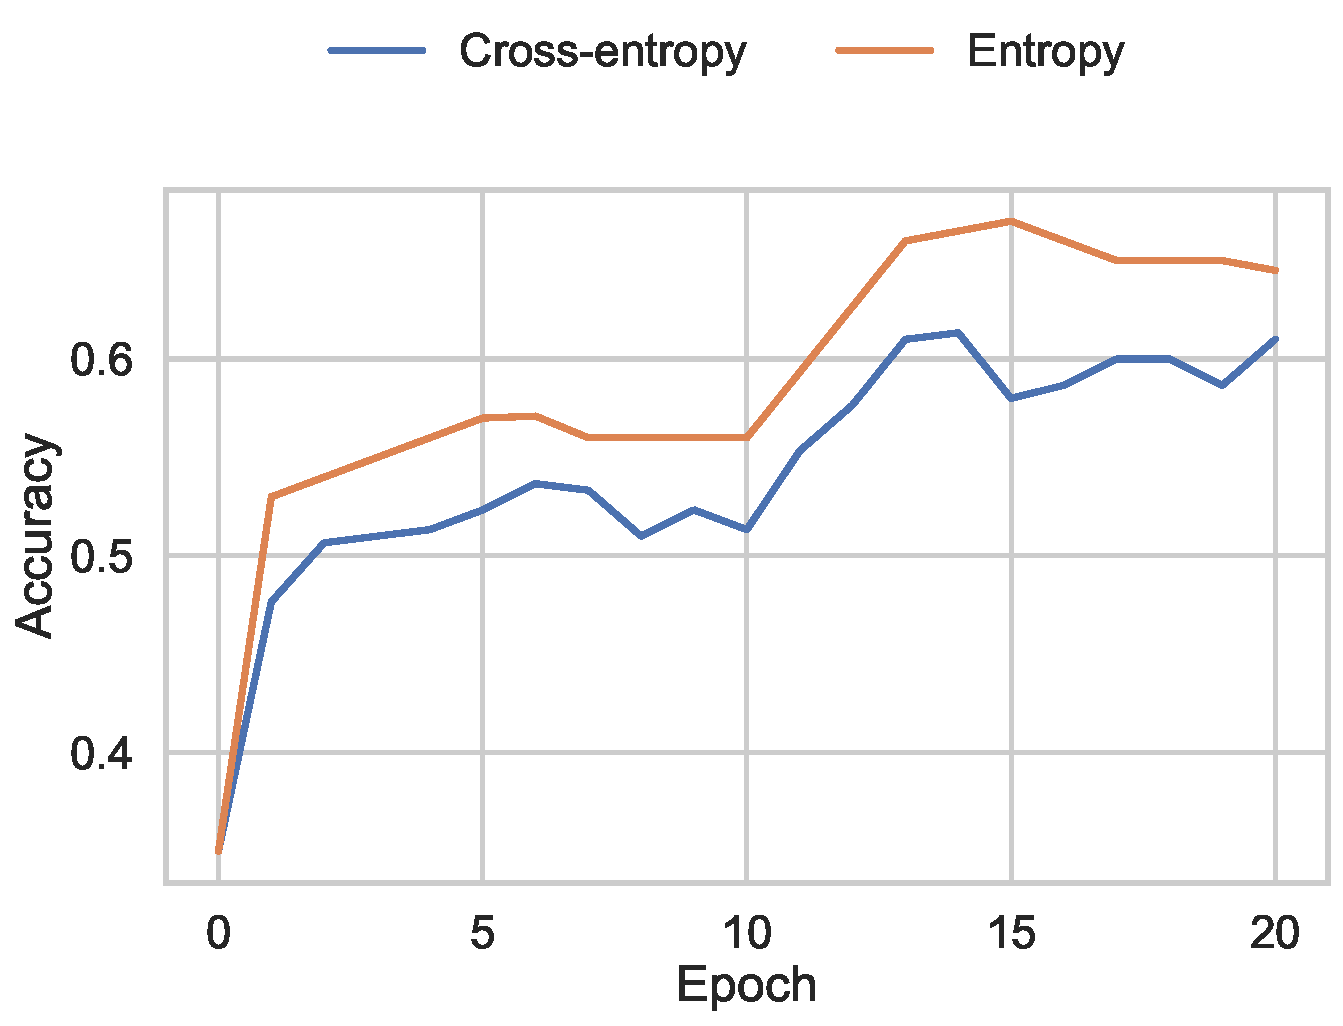
\includegraphics[width=\linewidth]{images/phi_e_vs_ce.pdf}
        \caption{Pipeline performance with cross-entropy (Phi-4-mini)}
        \label{fig:entropy_vs_crossentropy__phi4mini}
    \end{subfigure}
    \caption{Pipeline complexity metric performance comparison for entropy and cross-entropy across Phi-4-mini and Qwen 3B models.}
    \label{fig:entropy_vs_crossentropy_analysis}
\end{figure}

Figures \ref{fig:entropy_vs_crossentropy_qwen3B} and \ref{fig:entropy_vs_crossentropy__phi4mini} show pipeline training results with cross-entropy as a complexity metric compared to entropy. We observe comparable results for Qwen 3B, while Phi4-mini demonstrates superior performance with entropy. The difference in performance could be attributed to entropy capturing the information across the entire distribution instead of a single correct token.

\begin{figure}[h]
    \centering
    \begin{subfigure}[b]{0.48\linewidth}
        \centering
        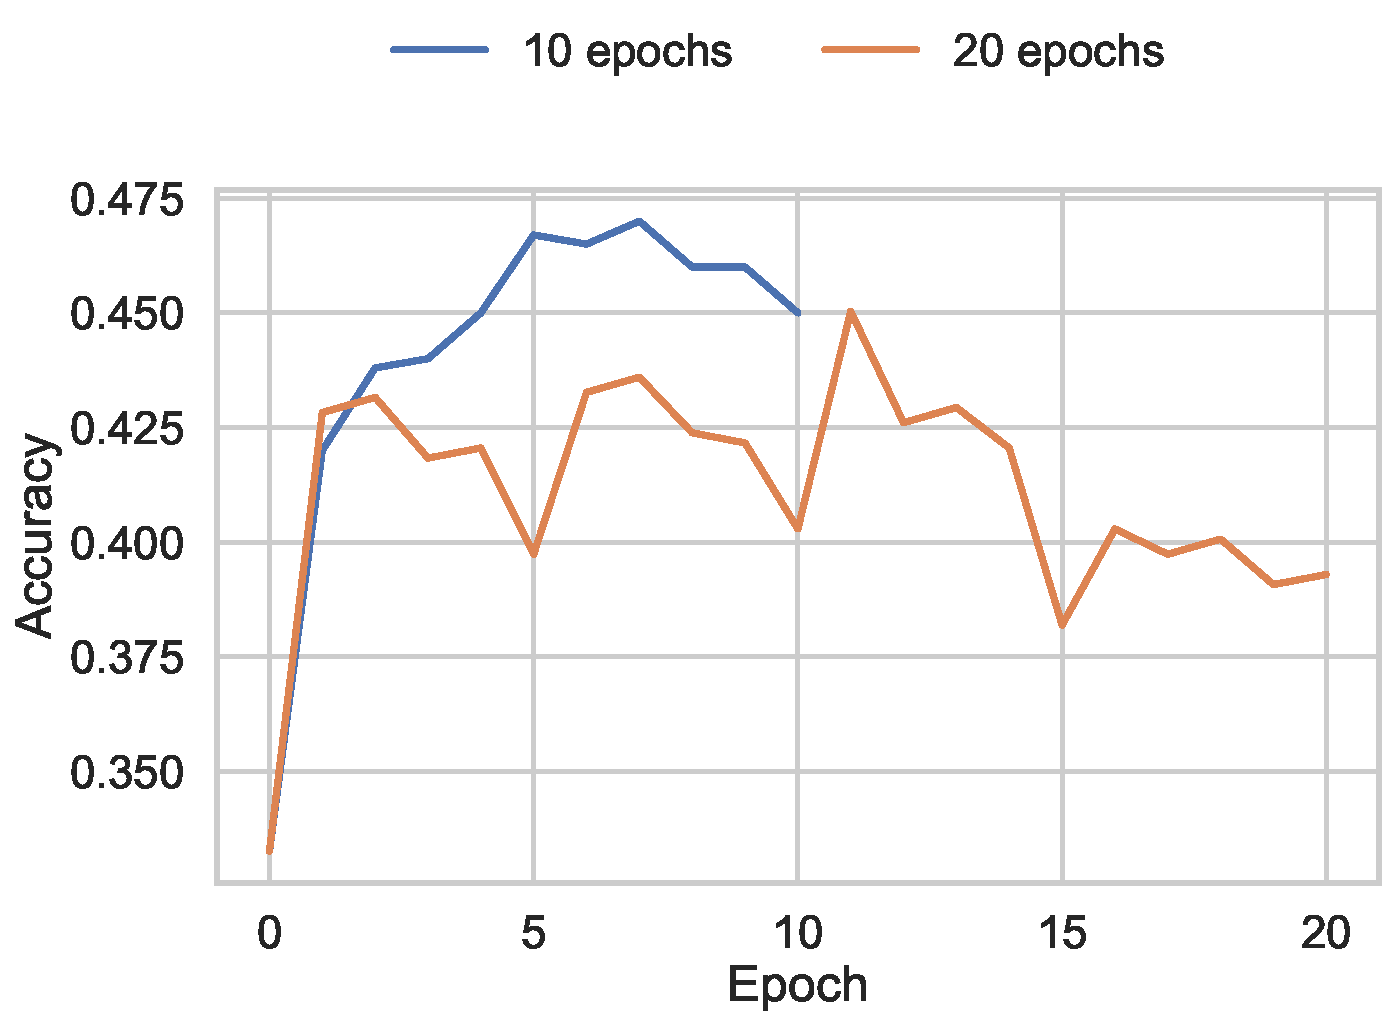
\includegraphics[width=1\linewidth]{images/qwen_sft_curriculum_comparison.pdf}
    \end{subfigure}
    \hfill
    \begin{subfigure}[b]{0.48\linewidth}
        \centering
        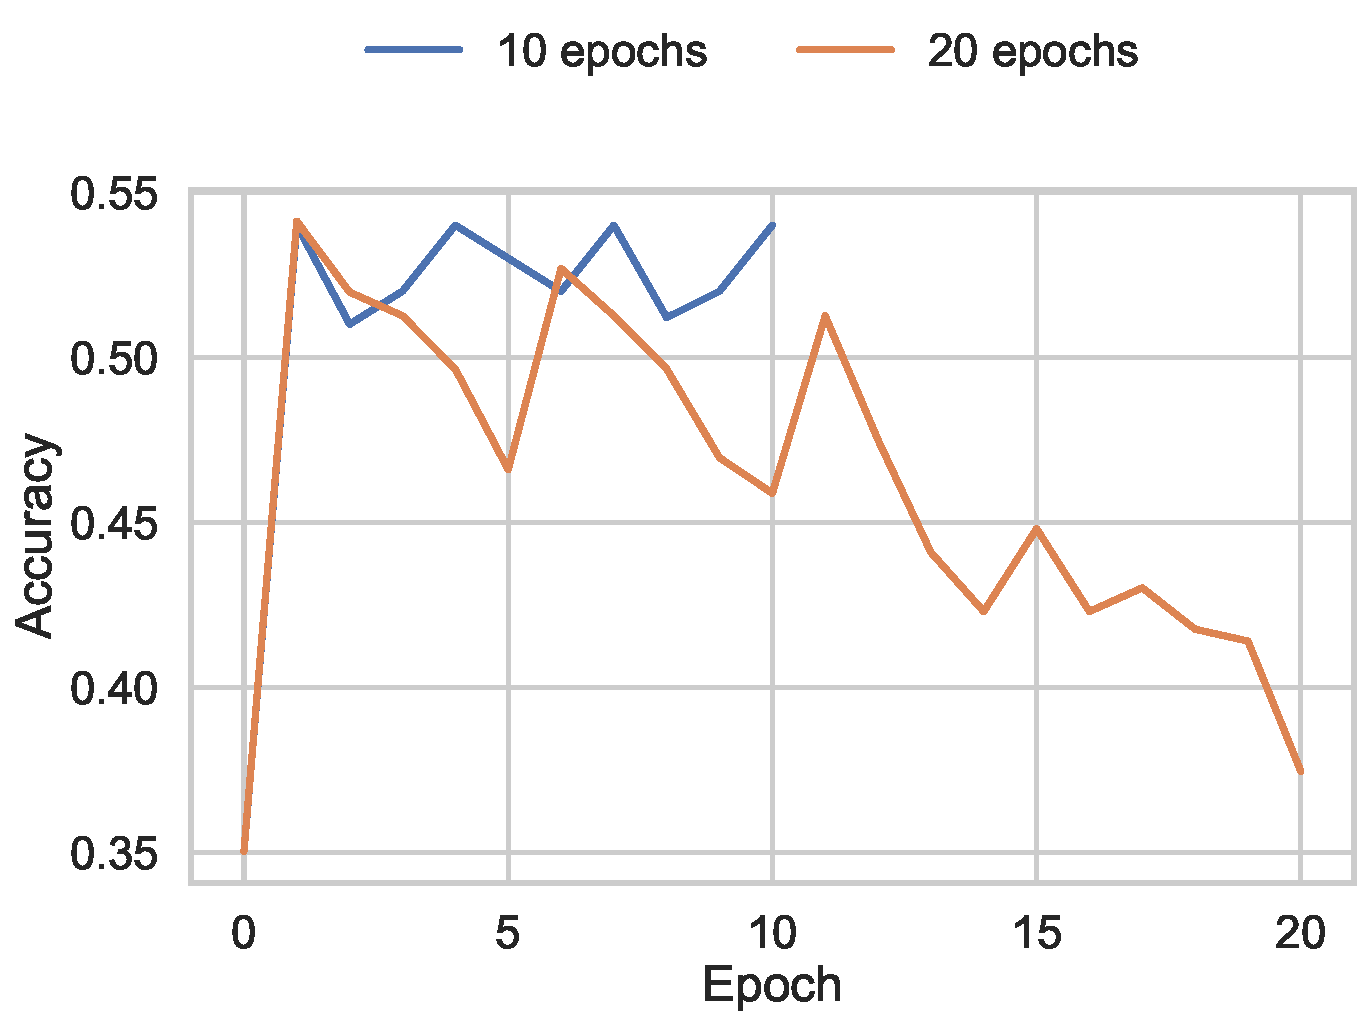
\includegraphics[width=1\linewidth]{images/phi_sft_curriculum_comparison.pdf}
    \end{subfigure}
    \caption{Curriculum learning accuracy dynamics for different models for Qwen 3B (left) and Phi-4-mini (right)}
    \label{fig:curriculum_plots}
\end{figure}

\begin{table*}[h]
    \centering
    \begin{subtable}[t]{0.48\linewidth}
        \centering
        \begin{tabular}{l c c c c}
            \hline
            Method & Qwen 3B & Phi4-mini \\
            \hline
            Without split & \textbf{0.72} / 0.70 & 0.72 / \textbf{0.74} \\
            \hline
            Education level \\
            \hline
            High school and easier & 0.73 / 0.72 & 0.76 / 0.75 \\
            Undergraduate & 0.73 / 0.71 & 0.72 / 0.77 \\
            Graduate & 0.66 / 0.65 & 0.64 / 0.68 \\
            Postgraduate & 0.63 / 0.52 & 0.64 / 0.63 \\
            \hline
            MASJ reasoning score \\
            \hline
            Low & 0.72 / 0.71 & 0.78 / 0.79 \\
            Medium & 0.72 / 0.70 & 0.70 / 0.72 \\
            High & 0.64 / 0.62 & 0.59 / 0.58 \\
            \hline
        \end{tabular}
        \caption{ROC AUC values for single-token response}
    \end{subtable}
    \hfill
    \begin{subtable}[t]{0.48\linewidth}
        \centering
        \begin{tabular}{l c c c c}
            \hline
            Method & Qwen 3B & Phi4-mini \\
            \hline
            Answer Entropy (AE) & 0.68 / 0.67 & 0.61 / 0.58 \\
            COT Mean & 0.59 / 0.58 & 0.59 / 0.63 \\
            COT Max & 0.63 / 0.61 & 0.6 / 0.65 \\
            Seq Mean & 0.6 / 0.59 & 0.6 / 0.62 \\
            Seq Max-Mean & 0.59 / 0.58 & 0.59 / 0.61 \\
            Seq Mean-Max & 0.62 / 0.6 & 0.59 / 0.62 \\
            Marg Diff Mean & 0.58 / 0.57 & 0.58 / 0.61 \\
            Top-2 Diff & 0.51 / 0.5 & 0.5 / 0.51 \\
            COT Max - AE & 0.54 / 0.53 & 0.51 / 0.57 \\
            COT Max + AE & 0.7 / 0.69 & 0.62 / 0.62 \\
            \hline
        \end{tabular}
        \caption{ROC AUC values for CoT response}
    \end{subtable}
    \caption{ROC AUC values for single-token and CoT responses}
    \label{tab:roc_auc}
    \footnotesize{Second result is for the alternative prompt to allow model answer "I do not know"}\\
\end{table*}

\subsubsection{Curriculum learning fragility}

Multi-stage pipelines such as curriculum learning show extreme sensitivity to hyperparameters such as the number of training epochs, learning rates, etc.

Figure \ref{fig:curriculum_plots} reveals the fragility of the original curriculum learning approach based on SFT. In this experiment, we train a model on the data with increasing complexity for 10 and 20 epochs with different splits: 
\begin{itemize}
    \item 10 epochs: 3 epochs on easy data, 3 epochs on medium data, and 4 epochs on hard data.
    \item 20 epochs: 5 epochs on easy data, 5 epochs on medium data, and 10 epochs on hard data. 
\end{itemize}
Qwen 3B plateaus at a lower accuracy with more training epochs, while Phi4-mini quickly overfits on the data, and its performance degrades.



\subsubsection{Quality of complexity estimation}

We consider three families of uncertainty estimation methods: MASJ, single-token entropy-based, and entropy-based augmented with a chain-of-thought.
MASJ results, as they are inferior to others, are provided in Appendix~\ref{sec:masj_evaluation}.

\paragraph{Single token and chain-of-thought answer entropy}

Table \ref{tab:roc_auc} presents the main ROC AUC values for single token entropy response and for the various aggregates of the chain-of-thought type of response. IDK responses and results with invalid formatting are excluded from the calculations. 

We see that the single-token response yields the best results. In-depth analysis of ROC AUC and accuracy scores with splits across domains and a larger selection of models can be found in tables \ref{tab:roc_auc_single_token_entropy} and \ref{tab:roc_auc_cot_entropy} in the Appendix.

Key observations include:
\begin{itemize}
    \item Single token response provides the best ROC AUC score. At the same time, 'IDK' responses do not consistently affect ROC AUC for all models.
    \item Accuracy tends to be slightly higher when an LLM can answer 'IDK'.
    \item Chain-of-thought responses tend to provide higher accuracy, but lower ROC AUC scores, which makes them less suitable for complexity estimation.
    \item Maximum-based measures (COT Max, Seq Mean Max) consistently outperform mean-based approaches (COT Mean, Seq Max Mean and Seq Mean Mean), suggesting peak uncertainty moments may better indicate question difficulty than average uncertainty.
    \item The poor close-to-random performance of the difference in top entropies suggests that modern LLMs maintain relatively stable reasoning to outliers.
    \item Sequence-based methods did not show good improvements over basic aggregation, indicating that modeling the reasoning structure provides marginal benefits.
\end{itemize}

% \begin{table*}
% \centering
% \begin{tabular}{l c c c c}
% \hline
% Method & Qwen 3B & Qwen 3B* & Phi4-mini & Phi4-mini* \\
% \hline
% Answer Entropy & 0.68/0.36 & 0.67/0.34 & 0.61/0.22 & 0.58/0.17 \\
% COT Mean & 0.59/0.19 & 0.58/0.16 & 0.59/0.19 & 0.63/0.26 \\
% COT Max & 0.63/0.27 & 0.61/0.23 & 0.6/0.2 & \textbf{0.65}/0.3 \\
% Max COT and Answer Entropy Diff & 0.54/0.09 & 0.53/0.06 & 0.51/0.03 & 0.57/0.15 \\
% Sequence Mean Mean & 0.6/0.2 & 0.59/0.17 & 0.6/0.2 & 0.62/0.25 \\
% Sequence Max Mean & 0.59/0.18 & 0.58/0.16 & 0.59/0.18 & 0.61/0.22 \\
% Sequence Mean Max & 0.62/0.25 & 0.6/0.2 & 0.59/0.18 & 0.62/0.24 \\
% Marginal Diff Mean & 0.58/0.17 & 0.57/0.14 & 0.58/0.16 & 0.61/0.23 \\
% Top-2 Entropies Diff & 0.51/0.02 & 0.5/0 & 0.5/0 & 0.51/0.01 \\
% Hybrid Method & \textbf{0.7}/0.41 & \textbf{0.69}/0.37 & \textbf{0.62}/0.24 & 0.62/0.23 \\
% \hline
% Number of Samples & 11049 & 10724 & 9997 & 9973 \\
% \hline

% \end{tabular}
% \caption{ROC AUC / Gini results for COT response}
% \label{tab:roc_auc_cot_aggr_entropy}
% \footnotesize{* Alternative prompt to allow model answer "I do not know"}\\
% \end{table*}